\documentclass{beamer}
\usepackage{amsmath}
\usepackage{amssymb}
\usepackage{amsthm}
%\usepackage{physymb}
\usepackage{graphicx}
\usepackage{subcaption}
\usepackage{tikz, pgfplots, graphicx, standalone}
\iffalse
\setbeamertemplate{frametitle}
  {\begin{centering}\smallskip
   \insertframetitle\par
   \smallskip\end{centering}}
\setbeamertemplate{itemize item}{$\bullet$}
\setbeamertemplate{navigation symbols}{}
\setbeamertemplate{footline}[text line]{%
    \hfill\strut{%
        \scriptsize\sf\color{black!60}%
        \quad\insertframenumber
    }%
    \hfill
}
\fi

\definecolor{DarkFern}{HTML}{407428}
\definecolor{DarkCharcoal}{HTML}{4D4944}
\colorlet{Fern}{DarkFern!85!white}
\colorlet{Charcoal}{DarkCharcoal!85!white}
\colorlet{LightCharcoal}{Charcoal!50!white}
\colorlet{AlertColor}{orange!80!black}
\colorlet{DarkRed}{red!70!black}
\colorlet{DarkBlue}{blue!70!black}
\colorlet{DarkGreen}{green!70!black}

% Use the colors:
\setbeamercolor{title}{fg=Fern}
\setbeamercolor{titlelike}{fg=Fern}
\setbeamercolor{frametitle}{fg=Fern}
\setbeamercolor{normal text}{fg=Charcoal}
\setbeamercolor{block title}{fg=black,bg=Fern!25!white}
\setbeamercolor{block body}{fg=black,bg=Fern!25!white}
\setbeamercolor{alerted text}{fg=AlertColor}
\setbeamercolor{itemize item}{fg=Charcoal}
\newcommand{\dt}[1]{\frac{\mathrm d #1}{\mathrm dt}}
\begin{document}
\title{The Kuramoto Model}   
\author{\begin{tabular}{r@{ }l} 
Author:      & Manish Goregaokar, \\
Guide: 
             & Professor Punit Parmananda\\
Affiliation: & IIT Bombay
\end{tabular}} 
\date{\today} 

\frame{\titlepage} 


\frame{\frametitle{Coupled Oscillators} 

\begin{itemize}

\item Unidirectional \begin{align*}
\dt{\phi_1} &= \omega \\
\dt{\phi_2} &= \omega - k\sin(\phi_2 - \phi_1)
\end{align*}

\item Bidirectional \begin{align*}
\dt{\phi_1} &= \omega + k\sin(\phi_2 - \phi_1)\\
\dt{\phi_2} &= \omega - k\sin(\phi_2 - \phi_1)
\end{align*}
\end{itemize}
}
\frame{\frametitle{Synchronization}

\begin{figure}
\centering\
\includestandalone[mode=image,width=0.6\textwidth]{../i/detuning}

Perfect and imperfect synchronization
\end{figure}

}
\frame{\frametitle{Degree of synchronization}
\begin{figure}
\centering
\begin{subfigure}[b]{0.3\textwidth}
\centering
\includestandalone[mode=image,width=\textwidth]{../i/almostfull}
Almost full synchronization
\end{subfigure}\qquad\qquad
\begin{subfigure}[b]{0.3\textwidth}
\centering
\includestandalone[mode=image,width=\textwidth]{../i/partial}
Partial synchronization
\end{subfigure}

\centering
\begin{subfigure}[b]{0.3\textwidth}
\centering
\includestandalone[mode=image,width=\textwidth]{../i/nonesync}
No synchronization
\end{subfigure}
\end{figure}

}
\frame{\frametitle{The Kuramoto Model}

\begin{align*}\dot{\theta_i} &= \omega_i + \frac{K}{N}\sum_j a_{ij}\sin(\theta_j - \theta_i)\\
r &= \frac1{N}\left|\sum_i e^{i\theta_i}\right|
\end{align*}
\begin{itemize}
\item $\theta_i$ is the phase of oscillator $i$
\item $a_{ij}$ decides if two oscillators are coupled
\item $K$ is the coupling constant
\item $N$ is the number of particles
\item $\omega_i$ is the natural frequency of oscillator $i$
\item $r$ is the order parameter
\end{itemize}
}


\frame{\frametitle{Sample results}
\begin{figure}
\centering
\begin{subfigure}[b]{0.4\textwidth}
\centering
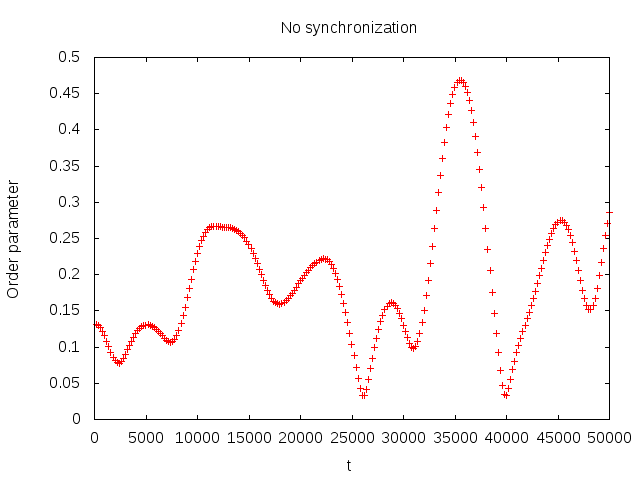
\includegraphics[width=\textwidth]{../data/strange}
\end{subfigure}
\begin{subfigure}[b]{0.4\textwidth}
\centering
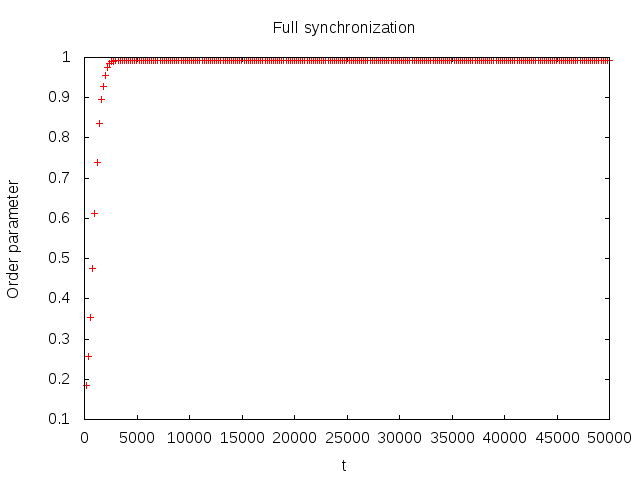
\includegraphics[width=\textwidth]{../data/full}

\end{subfigure}

\begin{subfigure}[b]{0.4\textwidth}
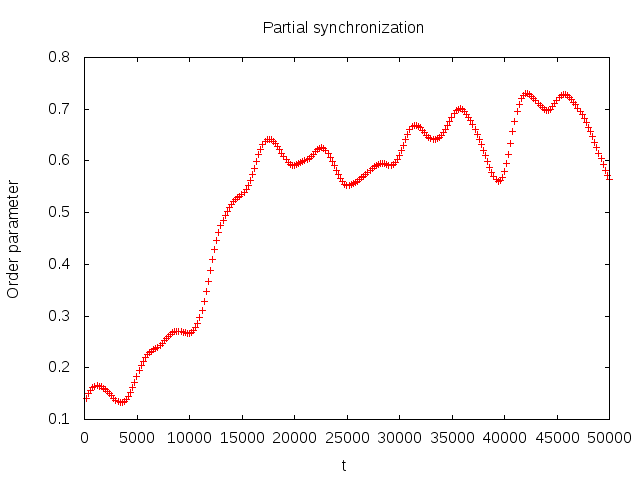
\includegraphics[width=\textwidth]{../data/partialsm}

\end{subfigure}
\begin{subfigure}[b]{0.4\textwidth}
\centering
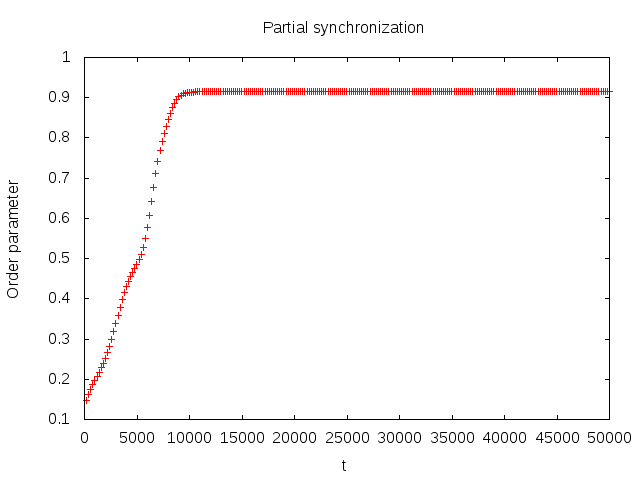
\includegraphics[width=\textwidth]{../data/partialmore}

\end{subfigure}
\end{figure}

}

\frame{
\begin{figure}
\centering
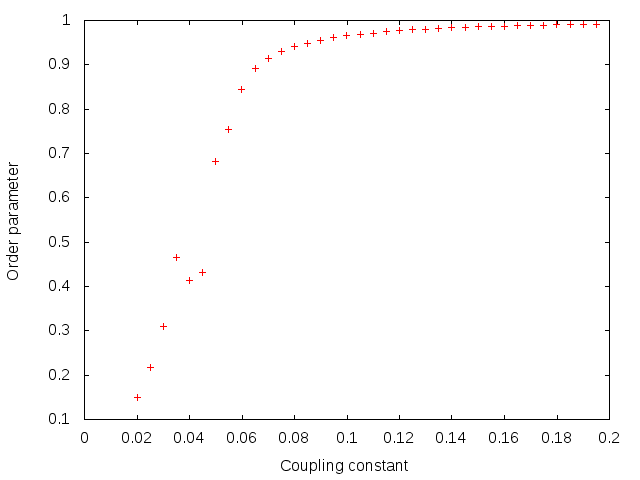
\includegraphics[scale=0.5]{../data/ovcoupling}

\end{figure}
}
\frame{
\begin{figure}
\centering
\includegraphics[scale=1]{../i/bifur}

\end{figure}
}
\end{document}

